\chapter{Results}\label{C:results}

This section examines the results of the bench marks. These results are in regard to the time taken, number of comparisons and the types of redundant tests identified. A range of the techniques discussed in Chapter \ref{C:workdone} will be examined, as discussed in the next section. 

In the tables below, a `+' represents that significant increase, `-' significant decrease and `=' represents no significant difference.

\section{Environmental Setup}

As previously discussed in Section \ref{performanceEvalBG} there are a variety of challenges that present themselves when using Java to evaluate the performance of a particular application. These challenges are discussed throughout the section.

\subsection{Distributed Grid Computing}
 A distributed grid computing system was used to execute the data analysis. This involved utilising idle computers located around Victoria University of Wellington's School of Engineering and Computer Science. A total of 150 jobs can be executed concurrently. If a user was to log on while a process was being conducted, the application would be paused until the user left.

\subsection{Measuring Time}
Java allows access to a system method that returns the total time in milliseconds from 1970 00:00:00 UTC to the current time. Calling this method before and after the analysing stage allows for the total time taken to analyse to be determined. However, the method has to execute, potentially causing the returned value to slightly off what it actually took. This is also true for the initial time, this time has to be returned and set assigned to a variable, causing a delay between when the analyse starts and the time stored. The time has minimal impact in the context of this framework and will be ignored. Using a distributed grid system has two effects. Firstly, using the system method would not be applicable as this would take into consideration when the application was not running. This was resolved by using the CPU time that the thread had used. Secondly, if a user logs in during analysis, the ram being used by the JVM could potentially be moved into virtual memory dependent on the amount of ram that the user needed. This was limited by running the tests at times when users were unlikely to log in such as overnight.

When measuring the time taken to analyse, the start up cost was not taken into account. Running up to 150 jobs meant that a large number of applications would be attempting to access a single data file at a single time. This involves a large level of non-deterministic behaviour, to avoid this, the start up cost was not considered.

\subsection{Hardware Environment}
\subsubsection{Heap Size}

The heap is the location that the JVM uses to store objects that are produced during the execution of an application. The heap is closely related to the GC. When the size of the heap increases, the number of objects that the garbage collector traverses increases in order to determine which objects should be collected. The amount of heap that was allocated to the JVM was 6gb for every benchmark over every run and was set through the grid system by requiring at least 6gb of free ram before running the process on that machine.

\subsubsection{Platform}

By using a distributed grid system, the platform required had to be specified. The platform that was used was a Linux 4.0.5 64 bit system with 8gb of ram. This was specified through the grid system such that every machine that was used to analyse the data met these requirements.

\subsection{Software Environment}
\todo{Number of VM invocations?}

A default garbage collection strategy was used. This is known as a concurrent-mark-sweep strategy which uses multiple threads to scan the heap, mark unused objects and recycle them \cite{oracle2015}. The approach allows for a high throughput but tends to use more CPU time than other strategies. This was deemed worth the trade off as memory was the bottleneck rather than CPU for the framework and increasing the throughput was more important.

\section{Method}

This section will go through the process of how the data was retrieved, analysed and evaluated.

Firstly, the benchmarks had to be set up in order to be run the tests locally. This involved retrieving the dependencies of each benchmark and setting up an build script through ant for each, in order to run the tests. After the tests had finished, the trace information was then saved to disk.

The data was then run on a grid computing setup. This setup involves a large number of computers which execute the instructions given to them.

Lastly, after the results had been returned, a Wilcoxon signed rank test was used to determine whether the results are significantly different or not. A Wilcoxon signed rank test is a paired difference test that compares two related samples. The significant level used is 95\%. A total of seven different property settings were run per benchmark. \todo{Should i want to put the settings for them in the appendices?} Each property setting was run 30 times. In this paper, the different combinations of techniques to identify redundancy will be as follows: 

\begin{itemize}
\item Pipeline size 2 vs Pipeline size 3
\item Parameters vs No Parameters
\item Weighting vs No Weighting
\item Weighting \& Parameters vs Neither
\end{itemize}

\section{Pipeline Length Comparison}
\todo{@DJ, I have set the figures and tables float specifier to 'H' to make it easier for you to read. Note, this is what is messing with the layout. I will fix for the final report.}
The significant table for comparing the use of pipeline of size two vs size three is shown in Table \ref{pipelinesig}. It shows that there was a mixture of results for the total time taken to analyse the data. Metrics-x, Ant, Spring and Jasm performed significantly better with a pipeline of size 3 in comparison to size two. Imcache had no significant difference and Whiley performed significantly worse with a pipeline of size three in comparison to size two. Every benchmark has no significant difference between the number of redundant tests identified, every benchmark produced the exact same number of redundant tests in both pipeline size of two and three.

A single pipeline comparison was left out due to the amount of memory that was required for it to be run. When using a list spectra, there could be up to several hundred thousand method calls for a test case and with thousands of tests this is a large amount of memory needed.

A chart showing how each benchmark reacted to the change in the pipeline size is shown in Figure \ref{fig:pipelinegraph}. It shows the number of comparisons that the final stage of the pipeline has to conduct.

\begin{table}[H]
\centering

\label{pipelinesig}
\begin{tabular}{|l|l|l|}
\hline
{\bf }          & {\bf Total Time} & {\bf Redundant Tests Identified} \\ \hline
{\bf Whiley}    & +                & =                           \\ \hline
{\bf Jasm}      & -                & =                           \\ \hline
{\bf Ant}       & -                & =                           \\ \hline
{\bf Spring}    & -                & =                           \\ \hline
{\bf Imcache}   & =                & =                           \\ \hline
{\bf Metrics-x} & -                & =                           \\ \hline
\end{tabular}
\caption{A table showing the significant relationship between the use of pipeline of size two with pipeline of size three for each benchmark}
\end{table}

\begin{figure}[H]
\begin{center}
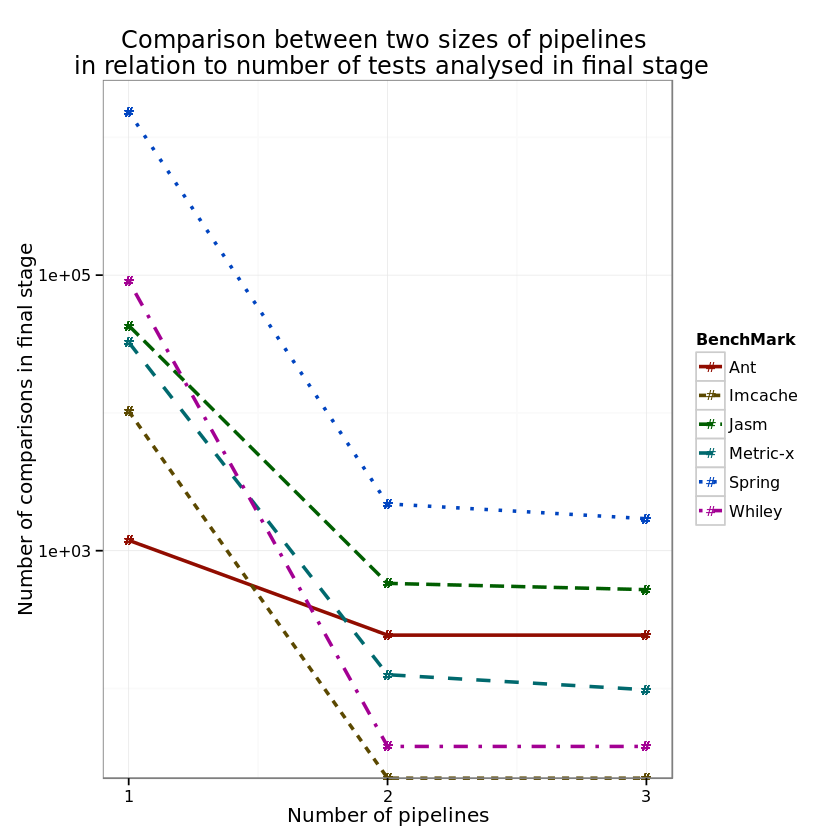
\includegraphics[height=10cm, width = 14.5cm]{Pipeline.png}
\end{center}
\caption{A figure showing the effect that using pipelines has on the number of comparisons that the final stage (Most computationally heavy) has to do.}
\label{fig:pipelinegraph}
\end{figure}


\section{K Length Comparison}
Figure \ref{fig:kdepthgraph} shows the change that the KDepth had on the number of redundant test cases identified. The amount of change is limited between one, two and three depth. Ant, Whiley and Spring appear to be the most responsive. \todo{Should I do sig test?}

\begin{figure}[H]
\begin{center}
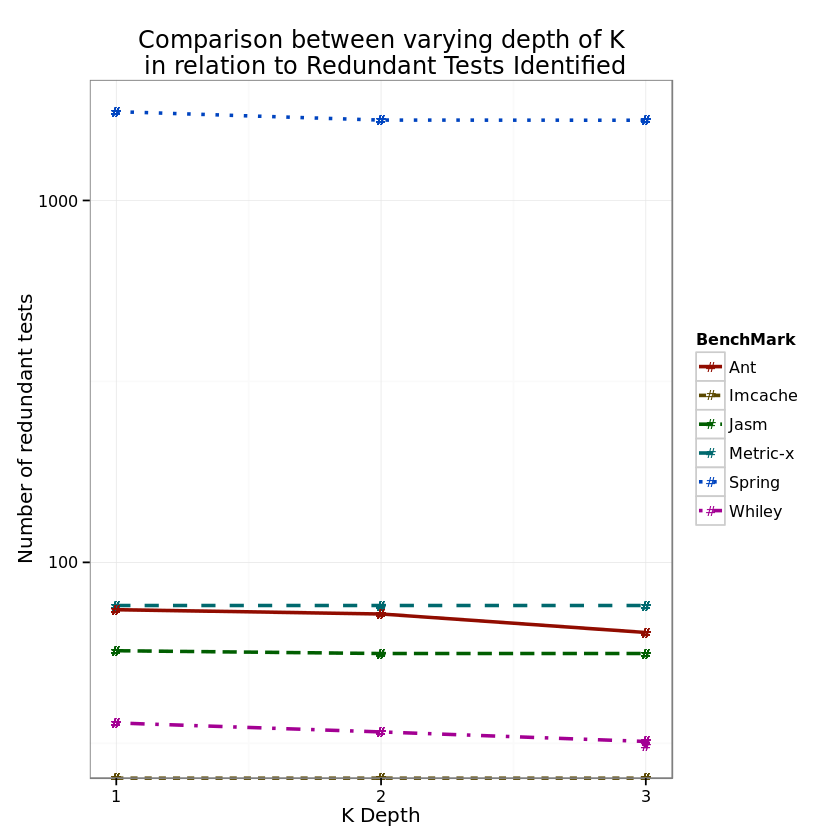
\includegraphics[height=10cm, width = 14.5cm]{KDepth.png}
\end{center}
\caption{A figure showing the effect that a change in the depth of the calling context has on the number of redundant tests are identified.}
\label{fig:kdepthgraph}
\end{figure}

\section{Parameter Comparison}

The significant table for comparing the use of parameters is shown in Table \ref{parametersig}. It shows that there was a negative relation for every benchmark in regard to time taken, this shows that parameters caused an increase in the time taken to analyse the data. Every benchmark had a significantly positive effect on the number of redundant test cases identified, showing that parameters decrease the number of redundant test cases. This is not the case in Imcache due to it having 0 redundant test cases identified in both, therefore no difference between the two.


\begin{table}[H]
\centering

\label{parametersig}
\begin{tabular}{|l|l|l|}
\hline
{\bf }          & {\bf Total Time} & {\bf Redundant Tests Identified} \\ \hline
{\bf Whiley}    & +                & -                           \\ \hline
{\bf Jasm}      & +               & -                          \\ \hline
{\bf Ant}       & +                & -                           \\ \hline
{\bf Spring}    & +                & -                           \\ \hline
{\bf Imcache}   & +                & =                           \\ \hline
{\bf Metrics-x} & +                & -                           \\ \hline
\end{tabular}
\caption{A table showing the significant relationship between the use of parameters and no parameters for each benchmark}
\end{table}

\begin{figure}[H]
\begin{center}
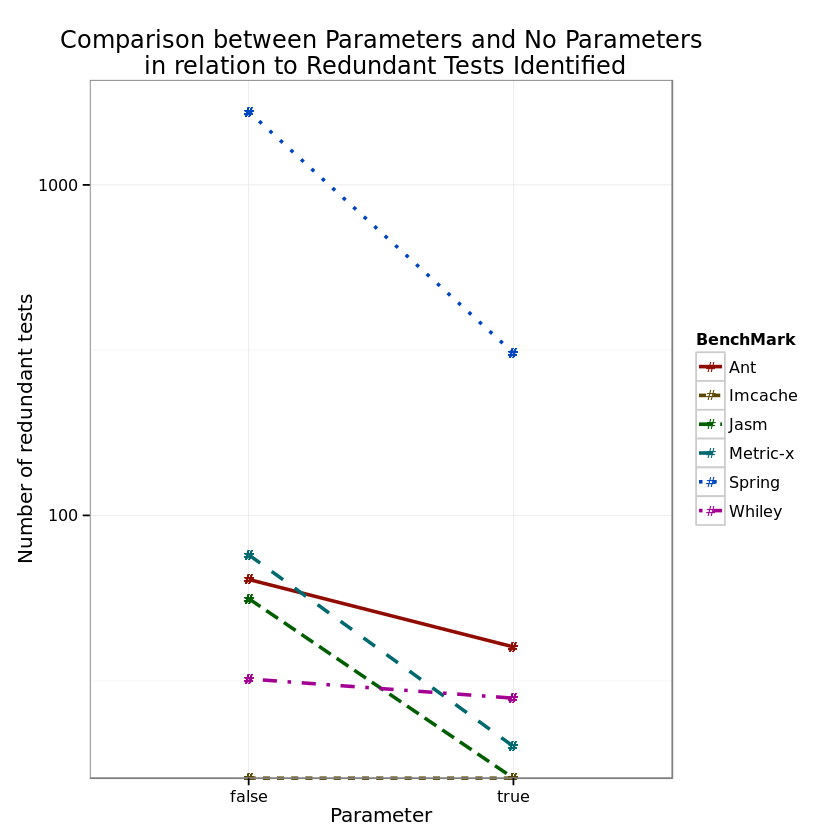
\includegraphics[height=10cm, width = 14.5cm]{Parameters.png}
\end{center}
\caption{A figure showing the effect that using parameters has on the number of redundant tests are identified.}
\label{fig:paramgraph}
\end{figure}

\section{Weighting Comparison}

The significant table for comparing the use of weighting is shown in Table \ref{weightingsig}. There are a mix for the benchmarks in regard to the total time taken to analyse the data. Whiley, Ant and Imcache had a significantly negative relation and weighting increased the time taken to analyse. Jasm, Spring and Metric-x had a significantly positive relation and weighting decreased the time taken to analyse. Whiley, Ant, Jasm and Metrics-x had a significantly positive relation in regard to the number of redundant tests identified, showing a decrease in the number identified when weighting was applied. Spring was the only benchmark where weighting had a significantly negative impact, increasing the tests identified.

\begin{table}[H]
\centering

\label{weightingsig}
\begin{tabular}{|l|l|l|}
\hline
{\bf }          & {\bf Total Time} & {\bf Redundant Tests Identified} \\ \hline
{\bf Whiley}    & +                & -                           \\ \hline
{\bf Jasm}      & -                & -                           \\ \hline
{\bf Ant}       & +                & -                           \\ \hline
{\bf Spring}    & -                & +                           \\ \hline
{\bf Imcache}   & +                & =                           \\ \hline
{\bf Metrics-x} & -                & -                           \\ \hline
\end{tabular}
\caption{A table showing the significant relationship between the use of weighting and no weighting for each benchmark}
\end{table}


\begin{figure}[H]
\begin{center}
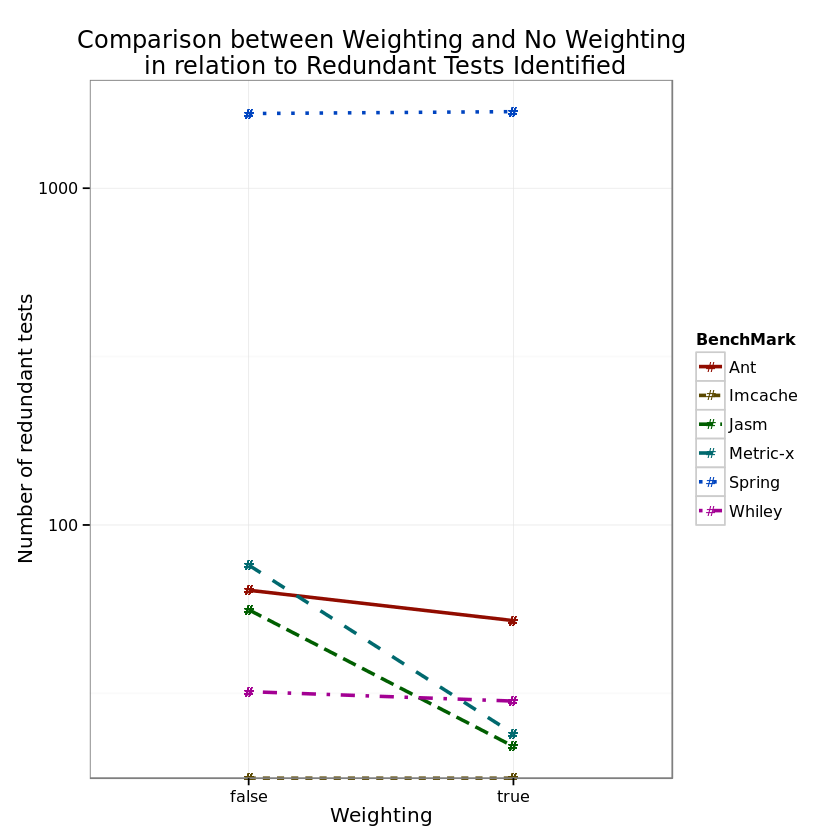
\includegraphics[height=10cm, width = 14.5cm]{Weighting.png}
\end{center}
\caption{A figure showing the effect that using weighting has on the number of redundant tests are identified.}
\label{fig:weightgraph}
\end{figure}

\section{Weighting and Parameter Comparison}

The significant table for comparing the use of weighting with parameters is shown in Table \ref{weightingparamsig}. It shows that for every Benchmark apart from Imcache, there was a negative relation for the time taken, showing that the time increased when using weighting and parameters for the majority of benchmarks. In contrast to this, every benchmark had a positive relation to the number of redundant tests identified.

\begin{table}[H]
\centering
\label{weightingparamsig}
\begin{tabular}{|l|l|l|}
\hline
{\bf }          & {\bf Total Time} & {\bf Redundant Tests Identified} \\ \hline
{\bf Whiley}    & +                & -                           \\ \hline
{\bf Jasm}      & +                & -                           \\ \hline
{\bf Ant}       & +                & -                           \\ \hline
{\bf Spring}    & +                & -                           \\ \hline
{\bf Imcache}   & -                & =                           \\ \hline
{\bf Metrics-x} & +                & -                           \\ \hline
\end{tabular}
\caption{A table showing the significant relationship between the use of weighting with parameters and neither for each benchmark}
\end{table}

\begin{figure}[H]
\begin{center}
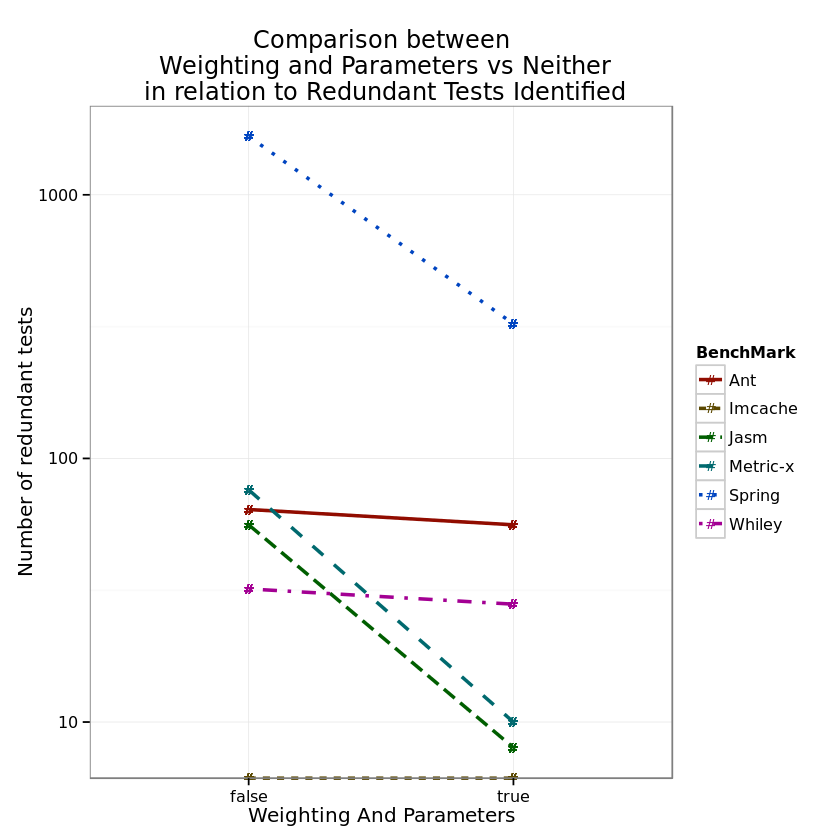
\includegraphics[height=10cm, width = 14.5cm]{WeightNParam.png}
\end{center}
\caption{A figure showing the effect that using weighting and parameters has on the number of redundant tests are identified.}
\label{fig:weightingparamgraph}
\end{figure}

\section{Redundant Test Case Coding}

Table \ref{whileycoding} and Table \ref{metriccoding} compare the four major variations of techniques used to show the different types of redundancy that were picked up for the Whiley and Metric-x benchmarks respectively. The tables show a list of codings, these codings are the types of redundancy that the framework identified. It is important to note that the numbers represent matching test cases, not redundant pairings. Such that there are 5 pairs that are the same, but 10 tests that match \todo{A bit counter intuitive, might need to redo to be pairing?}.

Table \ref{whileycoding} shows that the use of weighting removed the two test cases that had no redundancy, parameters removed the same as weighting as well as the different array value test cases and parameters and weighting combined matched the parameters. Table \ref{metriccoding} \todo{describe metric coding table}

\begin{table}[H]
\centering
\label{whileycoding}
\begin{tabular}{|l|l|l|l|l|}
\hline
                          & \multicolumn{4}{c|}{{\bf Whiley}}                                                             \\ \hline
{\bf Types of redundancy} & \multicolumn{1}{c|}{{\bf Pipeline 2}} & {\bf Weighting} & {\bf Parameters} & {\bf Parameters and Weighting} \\ \hline
Different Equation Value  & 6                                     & 6               & 6                & 6                \\ \hline
Different Equation Sign   & 8                                     & 8               & 8                & 8                \\ \hline
Different Array Values    & 2                                     & 2               & 0                & 0                \\ \hline
Same                      & 10                                    & 10              & 10               & 10               \\ \hline
Limited Redundancy        & 2                                     & 0               & 0                & 0                \\ \hline
Rearranged Equation       & 2                                     & 2               & 2                & 2                \\ \hline
Extra if statement        & 2                                     & 2               & 2                & 2                \\ \hline
                          &                                       &                 &                  &                  \\ \hline
{\bf Total}               & 32                                    & 30              & 28               & 28               \\ \hline
\end{tabular}
\caption{A table displaying a list of coding's for the Whiley Benchmark for four of the different techniques used.}
\end{table}

\begin{table}[H]
\centering
\label{metriccoding}
\begin{tabular}{|l|l|l|l|}
\hline
                          & \multicolumn{3}{c|}{{\bf Metric-X}}                   \\ \hline
{\bf Types of redundancy} & {\bf Weighting} & {\bf Parameters} & {\bf Parameters and Weighting} \\ \hline
Different Parameter Value & 10              & 8                & 4                \\ \hline
Different Object Type     & 2               & 2                & 0                \\ \hline
Different Array Values    & 6               & 4                & 6                \\ \hline
Similar                      & 2               & 0                & 0                \\ \hline
Limited Redundancy        & 4               & 6                & 0                \\ \hline
                          &                 &                  &                  \\ \hline
{\bf Total}               & 24              & 20               & 10               \\ \hline
\end{tabular}
\caption{A table displaying a list of coding's for the Whiley Benchmark for four of the different techniques used.}

\end{table}